\section{Exercise F}
\begin{enumerate}
    \item 
    In order to determine if a predicate logic formula is satisfiable, the tableau method can be used. By setting the root formula equal to true, it allows us to investigate the satisfiability of the formula. If all branches are closed, it means that there exists no interpretation of the formula that makes it true. Thus, the formula is not satisfiable. However, if a branch is open then there exists an interpretation of the formula that makes it true. Thereby making the formula satisfiable.  
    \item 
    This leaves the question of who shaves the barber? If he only shaves those who do not shave themselves, then he cannot shave himself, as then he, the barber, shaves someone who does shave himself breaking the fundamental rule. Furthermore, if he does not shave himself, then there is no one else to shave him, hence he cannot remain freshly shaved, breaking the fundamental rule that all the men in the town are shaved.
    \item The above situation can be translated into the following formula: \\
    $ \forall x (B(b,x) \leftrightarrow \neg B(x,x))$
\item 
Using the tableau method on the above formula:
\begin{center}
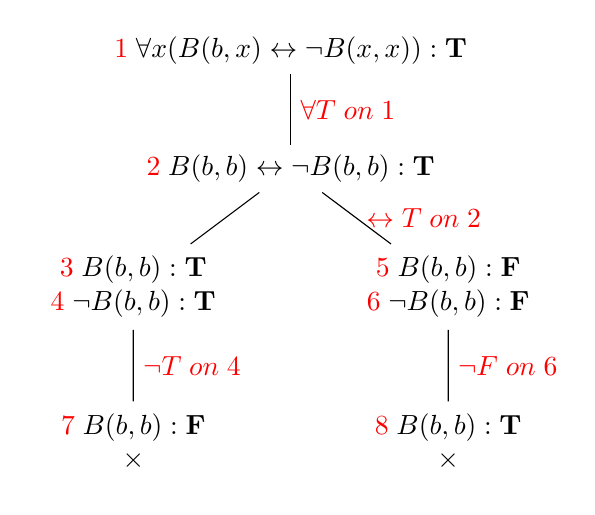
\begin{tikzpicture}

\node {$ \textcolor{red}{1}\; \forall x (B(b,x) \leftrightarrow \neg B(x,x)):\textbf{T} $} [sibling distance = 2cm] 
        child {node {$ \textcolor{red}{2}\; B(b,b) \leftrightarrow \neg B(b,b):\textbf{T} $} [sibling distance = 4cm] 
            child {node {$ \begin{array}{c} \textcolor{red}{3}\; B(b,b):\textbf{T} \\ \textcolor{red}{4}\; \neg B(b,b):\textbf{T} \end{array} $} [level distance=20mm]
                child {node {$ \begin{array}{c} \textcolor{red}{7}\; B(b,b):\textbf{F} \\ \times \end{array} $} 
                edge from parent node [right, red] {$\neg T\;on\; 4$}}}
            child {node {$ \begin{array}{c} \textcolor{red}{5}\; B(b,b):\textbf{F} \\ \textcolor{red}{6}\; \neg B(b,b):\textbf{F} \end{array} $} [level distance=20mm]
                child {node {$ \begin{array}{c} \textcolor{red}{8}\; B(b,b):\textbf{T} \\ \times \end{array} $}
                                    edge from parent node [right, red] {$\neg F\;on\; 6$}}
                                    edge from parent node [right, red] {$\leftrightarrow T\;on\; 2$}} 
                                    edge from parent node [right, red] {$\forall T\;on\; 1$}};

\end{tikzpicture}
\end{center}
It can be seen that the formula is not satisfiable because it does not have any open branches that could make it true. 
\end{enumerate}